\section{Data}

\subsection{Institutional Details}

The California Department of Transportation (Caltrans) is the department that
manages Aeronautics, Highway Transportation, Mass Transportation,
Transportation Planning, Administration, and the Equipment Service Center in
California. To outsource the labor for their highway construction projects,
Caltrans runs low-bid procurement auctions. Within the auctions, there are
typically large and small business bidders. Because small businesses have lower
economies of scale, their costs are higher compared to large businesses. Due to
the difference in costs, Caltrans grants ``bid preferences'' to the small
business bidders. Small businesses must meet three qualifications to be obtain
the Small Business Certification. The certification requires that the business
must be independently owned and operated in California, have no more than 100
employees, and over the last three tax years can only earn under \$10 million
average annual gross receipts. The benefit of the Small Business Certification
is that there is a higher probability of winning the auction. Once all bids are
submitted, the lowest bid wins the auction. However, if a small business’s bid
is within 5\% of the lowest bid, they win the auction and are awarded the
contract for construction. While the 5\% discount is used to determine the
winner, it is not applied to the actual amount the business is paid for the
project: Caltrans will pay the true price the winner bid.

\subsection{Data Overview}

% latex table generated in R 4.2.2 by xtable 1.8-4 package
% Tue Feb 21 10:13:43 2023
\begin{table}[ht]
\begin{tabular}{rrrrr}
  \toprule
 & Mean & Standard Deviation & Minimum & Maximum \\ 
  \midrule
Bids & 986241.65 & 3311628.21 & 44655.00 & 58547700.00 \\ 
  Small Business Bids & 531334.61 & 723168.10 & 49650.00 & 15485561.50 \\ 
  Number of Bidders & 5.70 & 3.18 & 1.00 & 20.00 \\ 
  Engineer's Estimates & 943980.19 & 3734611.68 & 74000.00 & 60058000.00 \\ 
  Workday & 94.28 & 155.89 & 8.00 & 1430.00 \\ 
   \bottomrule
\end{tabular}
\end{table}

One immediate takeaway from this table is that small businesses are often
refusing to bid on larger contracts, given that their bids are both
much smaller on average and have a smaller standard deviation.

There were 705 auctions in total. On average there were 5.7 bidders in
each auction, and the average bid was 968,241.65.

We calculated the winning bids, see that on average, the winning bid was \$39,417 lower
than the state's cost estimate. This is a relatively small difference,
but it does suggest that competition among the bidders does drive the
procurement cost down for the state. It could also potentially
represent a winner's curse if the cost estimates are very accurate,
but this would require more analysis to confirm.

\subsection{Bidding Behavior}

%\lstinputlisting[firstline=38, lastline = 47]{./code/data.R}

First we estimated the true distribution of bids for large and
small businesses using kernel density estimation with a bandwidth
selected via leave-one-out cross-validation.
Kernel density estimation relies on the second derivative of the
density function, and will as a result tend to overestimate peaks and
underestimate valleys. We can see that in this plot, where
the density estimate is much higher than the first peak.

The large business bids do have a longer tail, which reflects that
they are more able to take on projects with a large cost than
the smaller businesses.

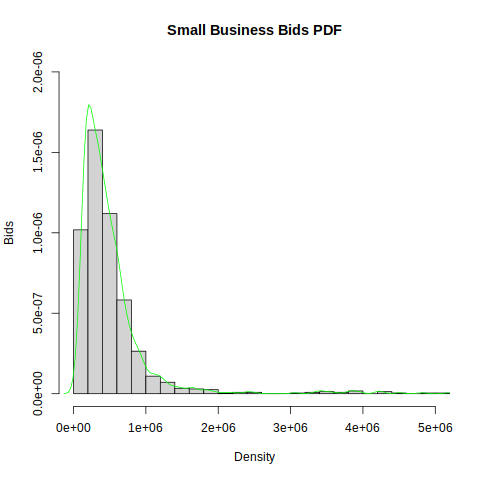
\includegraphics[scale=0.75]{sb-pdf.png}

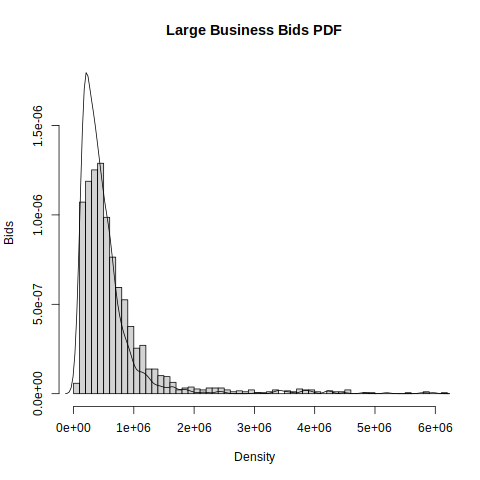
\includegraphics[scale=0.75]{lb-pdf.png}

Because of the data's skew, we applied a log transformation to
normalize the data and provide a better visualization of the long tail.
This reveals a very slight bimodal peak around bids of about \$3 million,
which might be a common project cost.

% \lstinputlisting[firstline=49, lastline = 61]{./code/data.R}

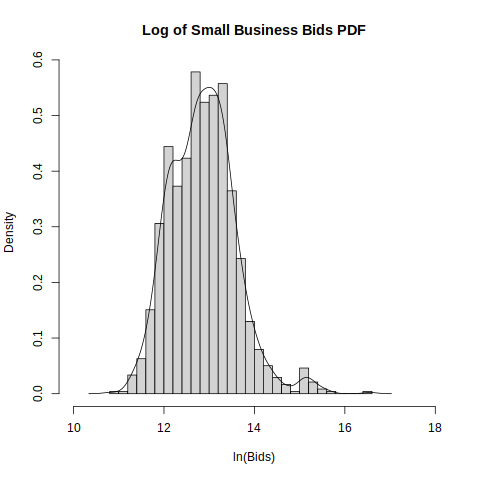
\includegraphics[scale=0.75]{log-sb-pdf.png}

We also plotted the CDFs to see patterns in the bid sizes between
the two types of bidders. The smaller average bids of
the small businesses are very clear in this plot, as the line is strictly
greater than the large businesses' estimated CDF.

% TODO: these line numbers will change
% \lstinputlisting[firstline=63, lastline = 80]{./code/data.R}

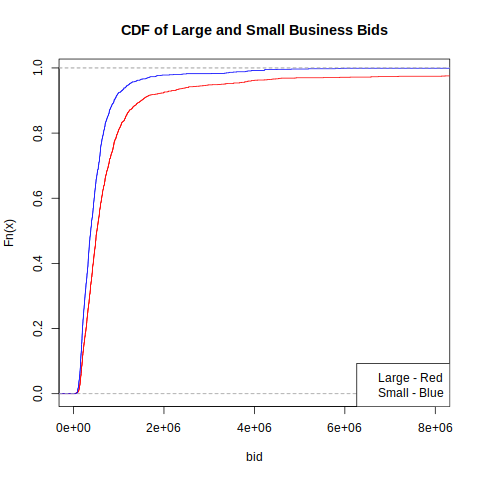
\includegraphics[scale=0.75]{cdf.png}

\subsubsection{Regressions}

present the estimates in a table properly labled.

To better understand the bidding behavior of business, we ran regressions on
bidders, engineer’s estimate, and work days. Bidders is how many bidders there
were for a certain project, engineer’s estimate is the estimate on how much a
professional believes the project costs, and work days is how long the project
will take. The first regression we ran included both small and large
businesses, and below is the result.

\[
\text{Bid} = -18,820 \text{Bidders} + 0.849 \text{Engineer’s Estimate} +
716 \text{Work Days} + 224,200
\]

% latex table generated in R 4.2.2 by xtable 1.8-4 package
% Tue Feb 21 10:37:37 2023
\begin{table}[ht]
\begin{tabular}{rrrrr}
  \toprule
 & Estimate & Std. Error & t value & Pr($>$$|$t$|$) \\ 
  \midrule
(Intercept) & 224239.4332 & 32012.8642 & 7.00 & 0.0000 \\ 
  num\_bidders & -18815.3332 & 4617.4432 & -4.07 & 0.0000 \\ 
  Estimate & 0.8494 & 0.0041 & 205.05 & 0.0000 \\ 
  WorkDays & 715.9631 & 99.6008 & 7.19 & 0.0000 \\ 
   \bottomrule
\end{tabular}
\end{table}

The results of this regression are as we expected. The negative sign on bidders
is consistent with the theory we studied, because with more bidders in a
particular auction, it drives down the price of the bid.

Further as the engineer’s estimate increases, the bid should
increase because there is a higher cost for the project. Finally, as work days
increases, so should the bid because it is a more expensive project as it takes
longer. The next regression we ran contains the same variables, except it only
includes small business bidders. The results are below.

\[
\text{Bid} = -16,470 \text{Bidders} + 0.9496 \text{Engineer’s Estimate} +
154.3 \text{Work Days} + 135,200
\]

These results also have the same signs as we expected for the same reasons as
above. The only difference in this regression is the degree to which work days
influences the bid. The coefficient for the regression with only small business
bidders is 154.3 compared with 716 for the regression including all businesses.
This might indicate that number of work days does not increase the bid as much
because smaller businesses might not be able to handle the cost of larger
projects that require more time and capital. Therefore, they can’t bid as high.

The next regression includes the same variables again, except it only focuses
on large business bidders.

\[
\text{Bid} = -22250 \text{Bidders} + 0.8398 \text{Engineer’s Estimate} +
1372 \text{Work Days} + 183900
\]

This regression also follows the same signs as we expected. The one difference
in this regression is the bigger coefficient for work days, such that there is
a much larger coefficient on work days for large business bidders. This can be
explained by the fact that large businesses can handle the higher costs of
lengthier projects. Their economies of scale allow for them to afford projects
that require more time and capital. Because of this, they are more likely
to pursue such projects and can bid higher for them.

